\documentclass[letterpaper,11pt]{article}

\setlength{\voffset}{0.1in}
\setlength{\paperwidth}{8.5in}
\setlength{\paperheight}{11in}
\setlength{\headheight}{0in}
\setlength{\headsep}{0in}
\setlength{\textheight}{11in}
\setlength{\textheight}{9.5in}
\setlength{\topmargin}{-0.25in}
\setlength{\textwidth}{7in}
\setlength{\topskip}{0in}
\setlength{\oddsidemargin}{-0.25in}
\setlength{\evensidemargin}{-0.25in}

\usepackage{xunicode}
\usepackage{xltxtra}
\XeTeXlinebreaklocale "zh"
\XeTeXlinebreakskip = 0pt plus 1pt
\setsansfont{AR PL UKai CN}
\setromanfont{AR PL UKai CN}

%\usepackage{fullpage}
\usepackage{shading}
%\textheight=9.0in
\pagestyle{empty}
\raggedbottom
\raggedright
\setlength{\tabcolsep}{0in}
\usepackage{sphinx1}
\usepackage{picins}
\usepackage{graphicx}
%-----------------------------------------------------------
%Custom commands
\newcommand{\resitem}[1]{\item #1 \vspace{-2pt}}
\newcommand{\resheading}[1]{{\large \parashade[.9]{sharpcorners}{\textbf{#1 \vphantom{p\^{E}}}}}}
\newcommand{\ressubheading}[4]{
\begin{tabular*}{6.5in}{l@{\extracolsep{\fill}}r}
        \textbf{#1} & #2 \\
        \textit{#3} & \textit{#4} \\
\end{tabular*}\vspace{-2pt}}
%-----------------------------------------------------------

\begin{document}
\begin{tabular*}{7in}{l@{\extracolsep{\fill}}r}
\textbf{\Large 盛 艳}  & 手机: 13813147410\\
江苏省扬州大学 &  Email: \href{mailto:shengyan1985@gmail.com}{shengyan1985@gmail.com} \\
信息工程学院400173\# & 个人网站: \href{http://liz.appspot.com}{liz.appspot.com}\\
\end{tabular*}
\\

\vspace{0.1in}

\resheading{基本资料}
\parpic[r]{
  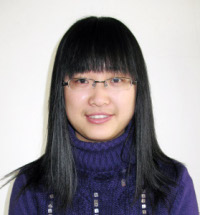
\includegraphics[height=4cm]{mypic.png}}
\begin{itemize}
\item {性别: }
女

\item {籍贯/出生年月: }
苏州/1985.08

\item {健康状况: }
良好

\item {毕业院校: }
\href{http://www.yzu.edu.cn}{扬州大学}, 信息工程学院

\item {专业及方向: }
计算机应用技术(数据挖掘)

\item {学历: }
硕士/2010年六月毕业

\end{itemize}


\resheading{教育经历}
\begin{itemize}
\item
    \ressubheading{硕士阶段}{}{2007年9月 - 现在}{}
    \begin{itemize}
        \resitem{   以优异成绩推荐免试于扬州大学信息工程学院, 攻读计算机应用技术专业/数据挖掘方向硕士学位;}
        \resitem{完成基础课程的学习, 主要有: 矩阵论, 数据仓库, 数据挖掘, 分布式数据库原理, 并行处理技术, 并行算法设计与分析, 计算机体系结构, 计算机网络技术, 最优化理论等; 同时进行相关理论研究工作, 主要关于文本数据挖掘, 概念格相关方向, 熟悉多种数据挖掘算法, 如: 经典Apriori, Decision Tree分类, 朴素贝叶斯分类, KNN分类, KMeans聚类, Rough Set Theory, Fuzzy Set Theory及形式概念分析中的Godin, Bordat算法等; 目前已发表多篇国内/国际学术论文, 并于2009年8月中旬参加ICNC-FSKD'09国际学术会议交流.}
    \end{itemize}
\item
    \ressubheading{本科阶段}{}{2003年9月 - 2007年7月}{}
    \begin{itemize}
        \resitem{   于扬州大学信息工程学院, 攻读计算机科学与技术(师范)专业学士学位;}
        \resitem{学习各门基础课程, 主要有: 高等数学, 概率论与数理统计, 线性代数, C/C++程序设计, 汇编语言, 数据结构, 操作系统原理, 编译原理, 计算机网络, 软件工程, 人工智能等, 取得优异成绩; 参加过2006年的ACM竞赛; 期间, 自学了Photoshop, Illustrator等图像处理软件; 并对Linux非常感兴趣, 从大三开始学习使用Linux操作系统(Ubuntu, Fedora).}
    \end{itemize}

\end{itemize}

\resheading{技能}

\begin{itemize}
\item{语言:}
掌握Python, C/C++, 熟悉 Java, \LaTeX ;
\item{操作系统:}
熟练使用Linux (Ubuntu, Fedora)的日常系统管理及维护;
\item{Web技术:}
熟悉Web应用开发; 熟练掌握Html, CSS, Javascript等Web技术, 并熟练使用 \href{http://jquery.com}{JQuery}, 有Ajax开发经验; 熟练掌握 \href{http://www.djangoproject.com/}{Django} 框架, 熟悉 \href{http://karrigell.sourceforge.net/}{Karrigell}, 熟悉GAE开发平台;
\item{数据库技术:}
掌握 \href{http://www.mysql.com}{MySQL}, \href{http://www.sqlite.org}{Sqlite3} 等数据库使用;
\item{系统管理:}
熟悉 Apache, Lighttpd等web服务器配置和管理; 熟悉ftp, svn, trac, samba等常见服务配置;
\item{其他:}
Photoshop, Illustrator图形/图像处理;
\item{英语水平:}
CET-4, 具有扎实的英语应用能力及较强的计算机专业英文文献阅读及翻译水平.
\end{itemize}

\resheading{项目经历}
\begin{itemize}

\item
    \ressubheading{Galicia平台扩展}{}{2007.9 - 2007.12}{}
    \begin{itemize}
        \resitem{   描述: Galicia是个开源项目, 在此基础上实现形式概念分析中的一些概念格构造算法, 如Godin算法, Godin改进算法等, 分析算法的时间空间复杂度.}
        \resitem{   职责: 在理解形式概念分析的基础上, 根据概念格自身特性, 掌握基本够格算法并实现, 之后图形显示结果格图, 以便更直观地得到概念格中概念及概念之间的继承关系.}
    \end{itemize}

\item
    \ressubheading{Openbookproject开放图书计划}{}{2008.4 - 2009.6}{}
    \begin{itemize}
        \resitem{   描述: 中文Pythonic技术图书的翻译编写项目, 其工程网址 \href{http://code.google.com/p/openbookproject/}{http://code.google.com/p/openbookproject}. 其中的LovelyPython是原创图书, 将Python以最易懂的方式介绍给读者.}
        \resitem{   职责: 参与LovelyPython图书编写过程, 参与部分章节的编写及校对等.}
    \end{itemize}

\item
    \ressubheading{禽流感病毒基因组生物信息学分析平台构建}{}{2008.11 - 2009.1}{}
    \begin{itemize}
        \resitem{   描述: 针对国际上各大生物信息中心提供的多个分析软件和基因/核酸数据库, 如BLAST检索系统及NCBI数据库, SMS2, Clustalx-2.0.10等, 进行本地化生物信息学分析平台的构建, 并在此基础上进行功能扩展, 方便科研人员对禽流感病毒基因进行分析.}
        \resitem{   职责: 完整搭建生物信息分析平台及其扩展. 主要有: 服务器基础环境安装及部署, 采用RedHat Enterprise Linux 4.0 AS作为服务器操作系统, 采用Apache2.2作为Web服务器及相关支持工具的安装. BLAST分析工具的本地化部署及相关数据库的安装, SMS2和Clustalx的安装部署, 并将三者整合起来. 其中, 基于Django0.96进行信息平台扩展并使用mod\_python部署到Apache上形成一整套完整的分析系统. 对系统扩展的工作主要有: 在所有基因数据库中提取禽流感病毒基因并构建二级数据库, 随着NCBI数据库的更新也随之更新并提供扩展检索功能.}
    \end{itemize}

\item
    \ressubheading{eachdn域名交易平台}{}{2009.5 - 2009.10}{}
    \begin{itemize}
        \resitem{   描述: 一个进行域名交易的电子商务网站, 其网址 \href{http://www.eachdn.com/}{http://www.eachdn.com}. }
        \resitem{   职责: 负责整个网站后台处理和部分前台设计, 包括需求分析, 数据库设计, 整体架构设计, 前台js设计等. 主要使用到的框架及技术有: Django, Mako, jQuery, Orbited, Xapian, Memcached等, 目前还在测试阶段.}
    \end{itemize}

\item
    \ressubheading{基于语义的协作信息检索框架研究}{}{2009.3 - 现在}{}
    \begin{itemize}
        \resitem{   描述: 此项目获得2009年江苏省高校研究生科研创新基金支持. 本项目研究如何设计一个利用语义的信息检索方案, 主要内容包括:1) 根据文本各个特征自身和类别信息的统计特性, 得到一种有效的文本特征提取方法; 2)基于概念格理论, 结合粗糙集理论和语义本体理论, 从形式概念的结构相似和语义相似两个层次上衡量概念间的相似度; 3)针对分布式环境, 提出并构建一个协作信息检索框架, 实现从结构和语义两个层次上的概念匹配, 获得更符合用户需求的检索结果. 4)在对检索结果排序过程中, 利用语义本体WordNet对用户历史检索记录进行分析, 从而构建用户兴趣模型, 并按照此模型对初始检索结果重新排序.}
        \resitem{   职责: 主持该项目, 阅读大量国内外学术论文, 研究文本特征提取方法和语义本体相关知识, 提出一种新的协作信息检索方案. 最后撰写并发表系列论文.}
    \end{itemize}
\end{itemize}

\resheading{发表论文}
\begin{itemize}
\item{2009 }
Yun Li, Yan Sheng, Luan Luan, Lianglei Sun and Ling Chen. A
Personalized Search Results Ranking Method Based on WordNet. The 5th
International Conference on Natural Computation(ICNC'09) and The 6th
International Conference on Fuzzy Systems and  Knowledge Discovery
(FSKD'09), Tianjin, China;

\item{2009 }
Li Yun, Sheng Yan, Luan Luan. A Text Classification Method with an
Effective Feature Extraction based on Category Analysis. The 5th
International Conference on Natural Computation(ICNC'09) and The 6th
International Conference on Fuzzy Systems and Knowledge Discovery
(FSKD'09), Tianjin, China;

\item{2008 }
SHENG Yan, LI Yun, TIAN Su-fang, LUAN Luan. A Rough Concept Lattice
Model of Variable Precision. IEEE International Symposium on
Intelligent Information Technology Application 2008 (IITA'08),
Shanghai City, China;
\item{2008 }
盛艳, 李云, 李拓, 栾鸾. 基于概念格模型的本体映射.
第三届江苏计算机大会(Jiangsu Computer Conference 2008, JSCC 2008);
此论文被评为第三届江苏计算机大会"优秀论文";

\item{2008 }
盛艳, 李云, 李拓, 袁运浩. 一种基于概念格模型的本体合并方法.
2008全国开放式分布与并行计算学术年会(DPCS2008);

\end{itemize}

\resheading{奖励/证书}
\begin{itemize}
\item{2003 - 2004学年 }
获一等专业奖学金;

\item{2003 - 2004学年 }
被评为院"三好学生";

\item{2004 - 2005学年 }
获二等专业奖学金;

\item{2004 - 2005学年 }
被评为校"三好学生";

\item{2005 - 2006学年 }
获朱敬文奖学金;

\item{2007学年 }
获"优秀毕业生"称号;

\item{2007 - 2008学年 }
获研究生朱敬文奖学金;

\end{itemize}

\resheading{兴趣}

\begin{itemize}
\item{生活: }
看经典电影; 听英文歌曲, 纯音乐; 打羽毛球; 喜欢涂鸦画画;

\item{计算机: }
喜欢使用各种图像处理软件和服务, 如PhotoShop, Illustrator, GIMP,
Picasa等; 关注IT新兴技术.

\item{学术研究: }
对智能信息检索, NLP中的方法和技术非常感兴趣;

\end{itemize}

\clearpage


\begin{tabular*}{7in}{l@{\extracolsep{\fill}}r}
\textbf{\Large Yan Sheng}  & Mobile Phone: 13813147410\\
Yangzhou University, JiangSu province &  Email: \href{mailto:shengyan1985@gmail.com}{shengyan1985@gmail.com} \\
400173\#, Institute of Information Engineering & Website: \href{http://liz.appspot.com}{liz.appspot.com}\\
\end{tabular*}
\\

\vspace{0.5in}

\resheading{Basic Info}
\begin{itemize}
\item {Sex: }
Female

\item {Origin/Birthday: }
SuZhou, China/1985, August

\item {Health status: }
Good

\item {Graduate institutions: }
Institute of Information Engineering,
\href{http://www.yzu.edu.cn}{Yangzhou University}

\item {Professional/Direction: }
Computer Application Technology/Data Mining

\item {Qualifications: }
Master/graduated in June 2010

\end{itemize}


\resheading{Education}
\begin{itemize}
\item
    \ressubheading{Master}{}{2007.09 - now}{}
    \begin{itemize}
        \resitem{   Studying in Institute of Information Engineering, Yangzhou University and doing some research about data mining;}
        \resitem{The courses I learned are: Matrix theory, data warehouse, data mining, distributed database theory, parallel processing, parallel algorithm design and analysis, computer architecture, computer network technology, optimization theory, etc; Do some research about data mining, concept lattice and be familiar with many data mining algorithms, such as: the classic Apriori, Decision Tree classifier, naive Bayesian classifier, KNN classifier, KMeans clustering, Rough Set Theory, Fuzzy Set Theory and Godin, Bordat algorithm in Formal Concept Analysis; Published many papers, and in mid-August 2009, participate in ICNC-FSKD'09 international academic conference.}
    \end{itemize}
\item
    \ressubheading{Bachelor}{}{2003.09 - 2007.07}{}
    \begin{itemize}
        \resitem{   Learned lots of things in Institute of Information Engineering, Yangzhou University and obtained the bachelor's degree of Computer Science and Technology;}
    \end{itemize}

\end{itemize}

\resheading{Skills}

\begin{itemize}
\item{Language:}
Python, C/C++, Java, \LaTeX ;
\item{OS:}
Linux (Ubuntu, Fedora);
\item{Web Technology:}
Use Html, CSS, Javascript and other Web technologies, \href{http://jquery.com}{JQuery}, also have Ajax development experience; Familiar with \href{http://www.djangoproject.com/}{Django} Web development framework and know about \href{http://karrigell.sourceforge.net/}{Karrigell}, GAE;

\item{Database:}
Familiar with \href{http://www.mysql.com}{MySQL}, \href{http://www.sqlite.org}{Sqlite} and other databases;

\item{System Maintain:}
Familiar with Apache, Lighttpd, ftp, svn, trac, samba;
\item{Other:}
Photoshop, Illustrator software;
\item{English:}
CET-4, have the good ability of English reading, writing, listening
and speaking. Do well in reading or translating English literature
of computer science and have published scholarly papers.
\end{itemize}

\resheading{Project Experience}
\begin{itemize}

\item
    \ressubheading{Galicia}{}{2007.9 - 2008.3}{}
    \begin{itemize}
        \resitem{   Describe: Galicia is an open source project to implement concept lattice construction algorithms.}
        \resitem{   Duties: Improve the Godin algorithms to obtain better time and space complexity.}
    \end{itemize}

\item
    \ressubheading{Openbookproject}{}{2008.4 - 2009.6}{}
    \begin{itemize}
        \resitem{   Describe: The project is about the translation or creatation of Chinese Pythonic book and the website is \href{http://code.google.com/p/openbookproject/}{http://code.google.com/p/openbookproject}. LovelyPython is a original book which aimed to introduce the python to reader in the most understandable way.}
        \resitem{   Duties: Took part in the writting process of LovelyPython.}
    \end{itemize}

\item
    \ressubheading{Construction of Avian virus genome bioinformatics analysis platform}{}{2008.11 - 2009.1}{}
    \begin{itemize}
        \resitem{   Describe: Since major international Bioinformatics Center provide many anaysis software for gene and gene/nucleic acid database, such as, BLAST retrieval system and NCBI database, SMS2, Clustalx-2.0.10, these analysis tools must be localized. Further more, some specail function need be extented, for instance, selecting and updating the Avian virus genome from the complete database.}
        \resitem{   Duties: We installed RedHat Enterprise Linux 4.0 AS as server operating systems, Apache2.2 as Web server and other utilities. After localizing the BLAST, SMS2 and Clustalx, we integrated three systems to one complete system. The main extension is selecting the Avian virus genome to build a sub-database which updates with the NCBI database.}
    \end{itemize}

\item
    \ressubheading{eachdn Domain Name Trading Platform}{}{2009.5 - 2009.9}{}
    \begin{itemize}
        \resitem{   Describe: An e-commerce website for domain name transactions, the website is \href{http://www.eachdn.com/}{http://www.eachdn.com}. }
        \resitem{   Duties: Responsible for the overall website's backend part, including needs analysis, database design, architecture design, including js. The main technologies and framework: Django, Mako, jQuery, Orbited, Xapian, Memcached and so on.}
    \end{itemize}

\item
    \ressubheading{Collaborative information retrieval research using semantic info}{}{2009.3 - now}{}
    \begin{itemize}
        \resitem{   Describe: This project was supported by Jiangsu Province Universities Research and Innovation Fund in 2009. The project is to design a information retrieval method using semantic info. The main contents contains: 1, design a new feature selection method; 2, advance an concept similarity measure based on concept lattice and rough set theory; 3, build a framework for collaborative information retrieval; 4, build a user interest model using WordNet and re-rank search results;}
        \resitem{   Duties: Read a number of papers, study of the text feature extraction methods, and semantic ontology-related knowledge, presents a new collaborative information retrieval method.}
    \end{itemize}
\end{itemize}

\resheading{Papers}
\begin{itemize}
\item{2009 }
Yun Li, Yan Sheng, Luan Luan, Lianglei Sun and Ling Chen. A
Personalized Search Results Ranking Method Based on WordNet. The 5th
International Conference on Natural Computation(ICNC'09) and The 6th
International Conference on Fuzzy Systems and  Knowledge Discovery
(FSKD'09), Tianjin, China;

\item{2009 }
Li Yun, Sheng Yan, Luan Luan. A Text Classification Method with an
Effective Feature Extraction based on Category Analysis. The 5th
International Conference on Natural Computation(ICNC'09) and The 6th
International Conference on Fuzzy Systems and Knowledge Discovery
(FSKD'09), Tianjin, China;

\item{2008 }
SHENG Yan, LI Yun, TIAN Su-fang, LUAN Luan. A Rough Concept Lattice
Model of Variable Precision. IEEE International Symposium on
Intelligent Information Technology Application 2008 (IITA'08),
Shanghai City, China;

\item{2008 }
Shengyan, Li yun, Li tuo, Luanluan. Ontology mapping based on the lattice model. Jiangsu Computer Conference 2008, JSCC 2008;

\item{2008 }
SHENG Yan, LI Yun, LI Tuo, YUAN Yun-hao. A method for ontology merging based on the concept lattice. DPCS2008;

\end{itemize}

\resheading{Interests}

\begin{itemize}
\item{Life: }
Like classical movies, listening English songs, drawing and playing badminton;

\item{Computer: }
Also like image processing software and services, such as PhotoShop, Illustrator, GIMP, Picasa. Concerned about the IT technologies;

\item{Research: }
interested in Intelligent Information Retrieval, NLP methods and techniques.

\end{itemize}

\clearpage

\end{document}
